\section{Introduction}
\subsection{Problem Background}

\begin{comment}
伴随着人类的发展,我们的生活水平和生活质量不断提高,但是在我们这个广大的世界之中,我们依然面临了诸多问题。联合国组织总结出了17个可持续发展的核心目标,这些问题有着不同的侧重点,但是他们都是我们最为重要的议题


联合国发展到今天,我们面临了许多问题这些问题有大有小,我们需要解决。
但同时,有一些问题伴随了人类历史这么多年,需要我们着重进行考虑。这些问题概括了人类历史发展的诸多问题挑战。他们有17个,我们称之为17个可持续发展问题。、
这些可持续发展问题有:
目标1:无贫困\\
目标2:零饥饿\\
目标3:良好的健康和福祉\\
目标4:优质教育\\
目标5:性别平等\\
目标6:清洁水和卫生\\
目标7:负担得起的清洁能源\\
目标8:体面的工作和经济增长\\
目标9:工业、创新和基础设施\\
目标10:减少不平等\\
目标11:可持续的城市和社区\\
目标12:负责任的消费和生产\\
目标13:气候行动\\
目标14:水下生命\\
目标15: 陆地生物\\
目标16:和平与正义强大的机构\\
目标17:实现目标的伙伴关系\\

如此之多的目标问题,我们需要进行分析,以便得到最终的解决方案,来让人类社会变得更加美好。
\end{comment}


The 17 Sustainable Development Goals (SDGs) are not standalone objectives, but rather a network of interdependent goals that interact with each other in various ways. The success of achieving one goal often depends on the success of achieving other goals. For instance, ensuring access to clean water and sanitation (SDG 6) is critical to reducing poverty (SDG 1) and improving health and well-being (SDG 3). Similarly, promoting affordable and clean energy (SDG 7) is essential to combatting climate change (SDG 13) and promoting sustainable cities and communities (SDG 11).

Conversely, the failure to achieve one goal can also hinder progress towards other goals. For example, if education (SDG 4) is not accessible to all, then achieving gender equality (SDG 5) and reducing poverty (SDG 1) become more difficult. Moreover, the failure to address climate change (SDG 13) may exacerbate hunger (SDG 2) and limit the availability of clean water and sanitation (SDG 6).

Therefore, it is essential to recognize the interconnectedness of the SDGs and address them holistically, rather than separately. To achieve sustainable development, we must prioritize integrated approaches that consider the impacts of achieving one goal on other goals. This requires collaboration and partnerships among governments, international organizations, civil society, and the private sector to develop strategies and implement solutions that address the interrelated challenges faced by the world. By working together and taking a systemic approach, we can achieve the SDGs and create a better world for all.



\begin{figure}[h]%插入图片并且加上图片的标题,这是一个模板
    \centering
    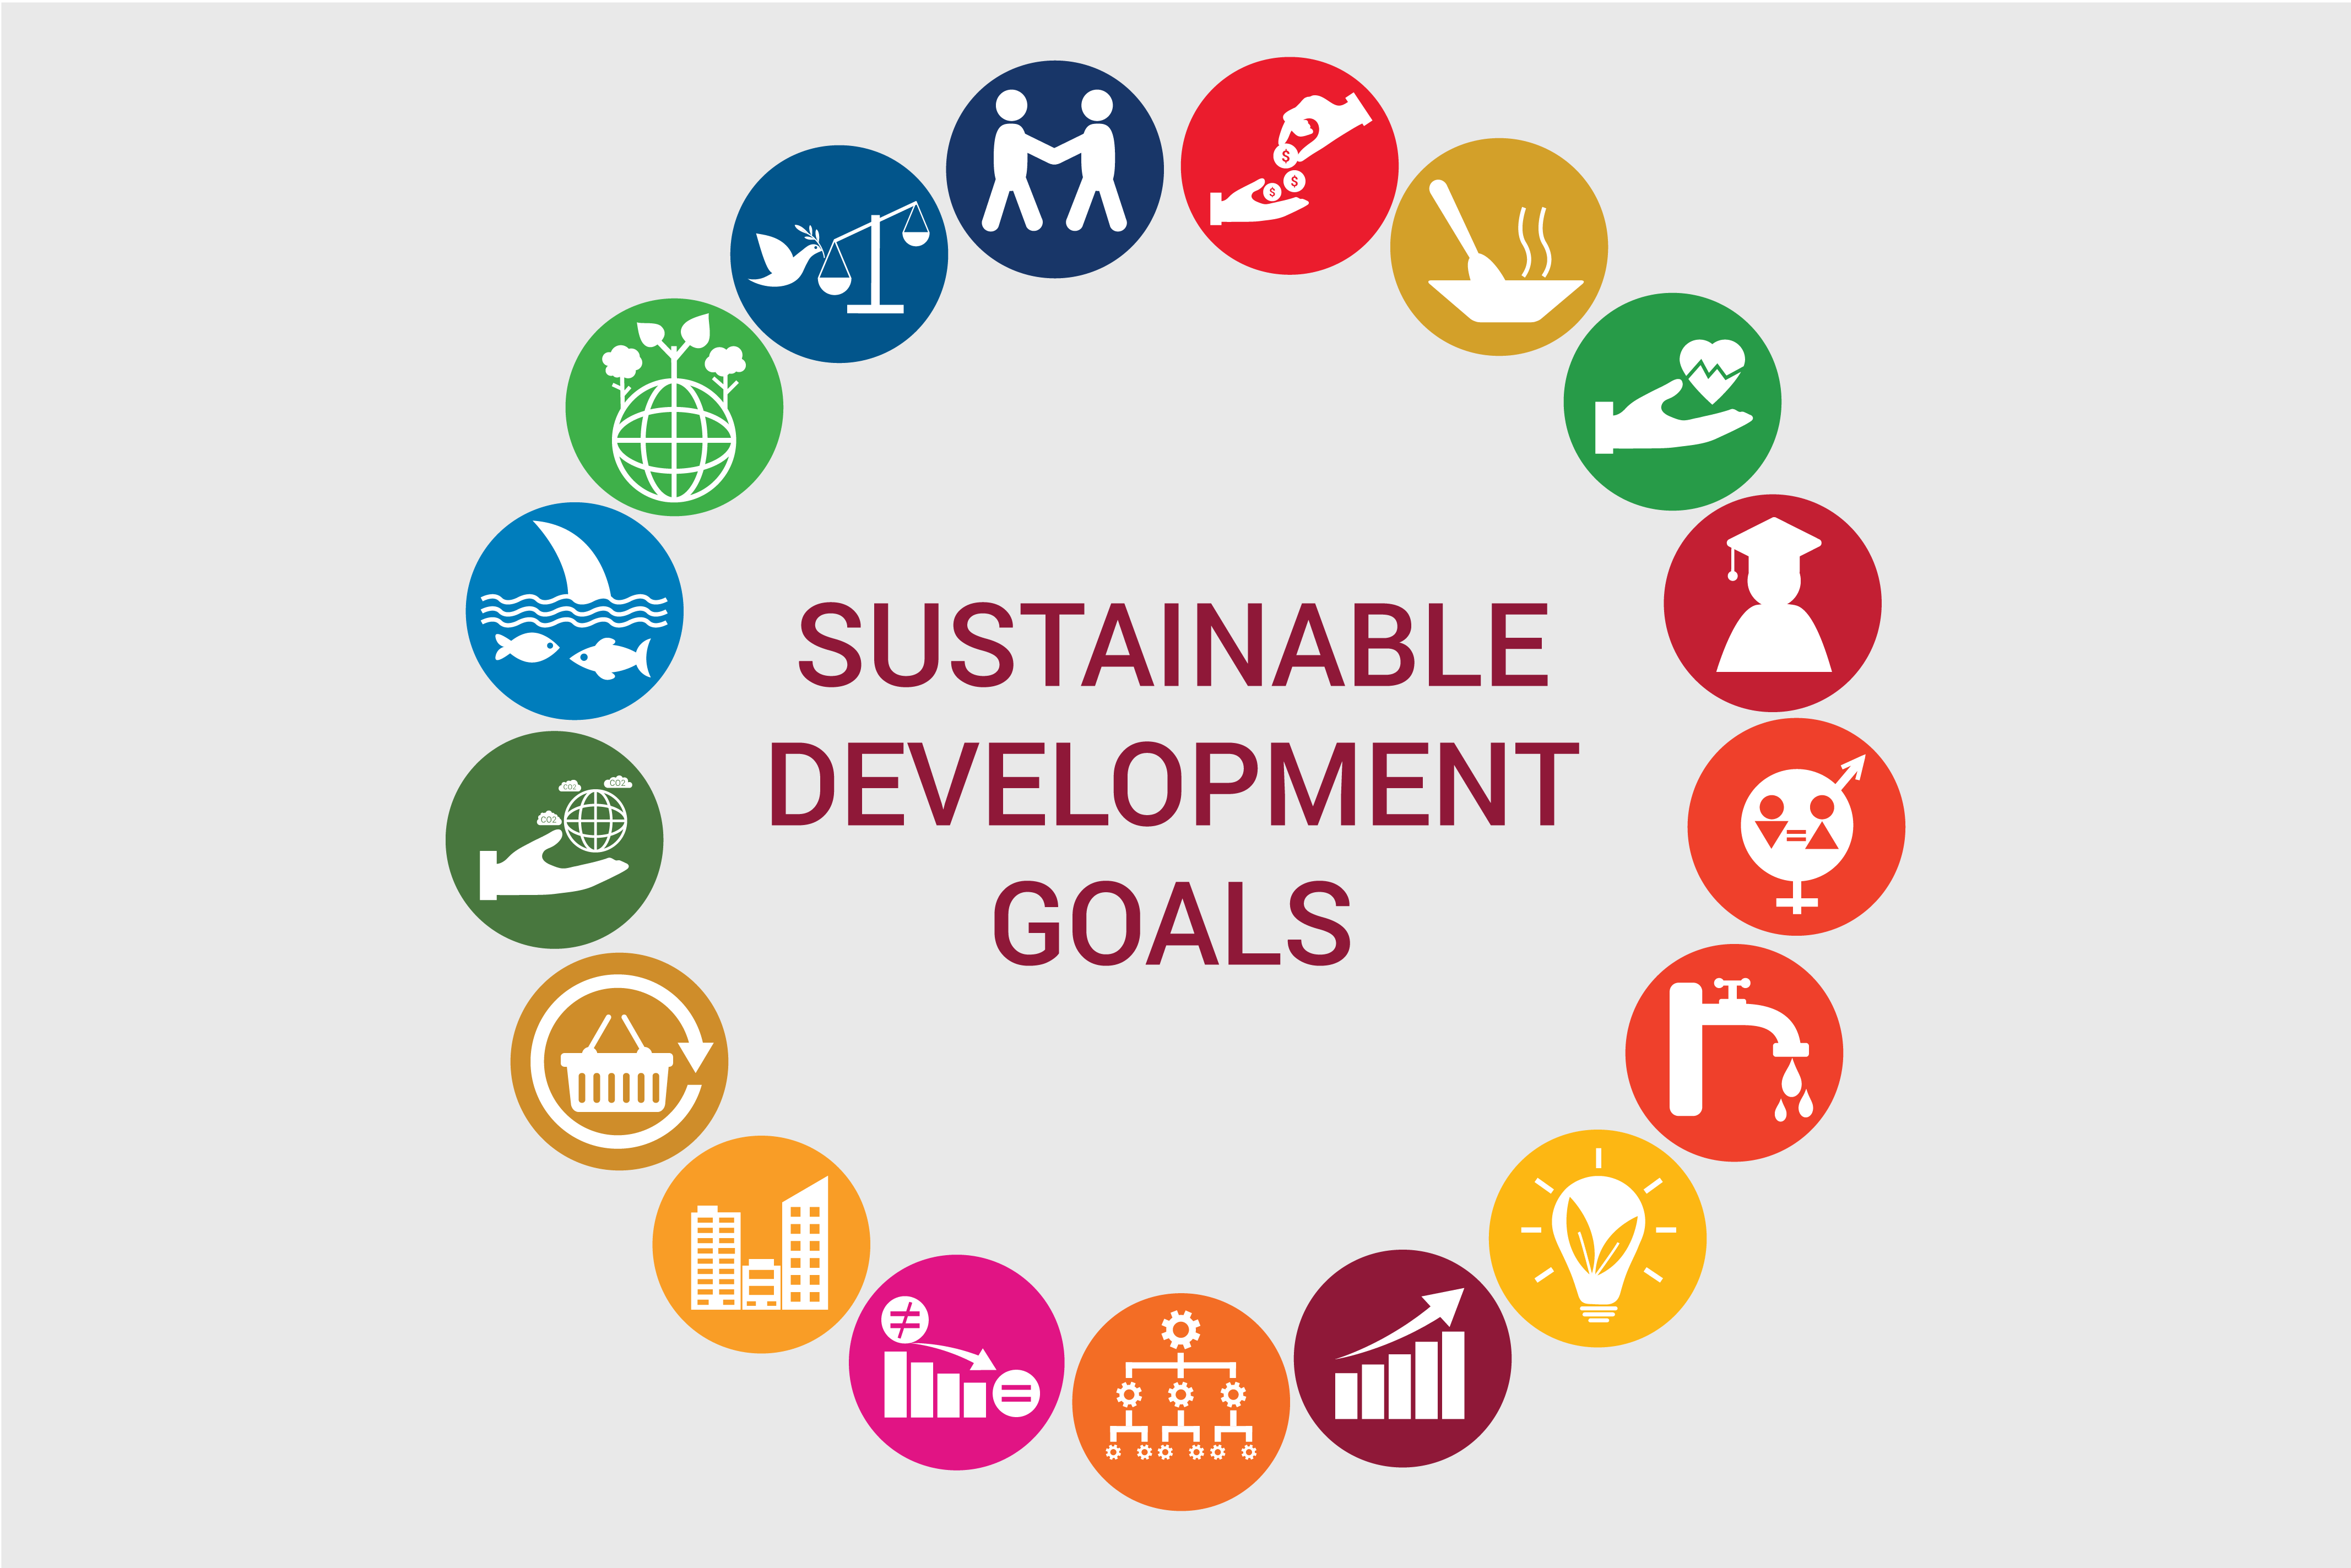
\includegraphics[scale=0.06]{{figure/SDGs.png}}%插入图片的指令
    \caption{The 17 SDGs of UN}%标题
    \label{Label}
\end{figure}



\subsection{Restatement of the Problem}



Considering the background information and restricted conditions identified in the problem statement, we need to establish a model that is universal in its applicability to different athletes and complete the following tasks using the model:    
\begin{itemize}
    \item \textbf{In Task 1} We need to create a \textbf{network} of relationships among the 17 SDGs. Since each of these 17 goal relationships has its own uniqueness, we treat each of the 17 goals as 17 nodes of the network and construct the undirected network. In a certain two nodes, i.e., between certain two goals, there is a unique relationship function. We indicate that they have certain connections by connecting lines in the relational network. The details are described in Task 1.
    
    
    \item In \textbf{Task 2}, We need to use the individual SDGs as well as the network structure to set priorities, and we need to prioritize each event. This task requires a generalization of the 17 SDGs, as well as a decision model that can effectively calculate priorities and make stage-by-stage projections of future development trends.
    

    \item In \textbf{Task 3}, We need to test the scalability of the model. We need to consider how the structure of our network will change when one of the SDGs is achieved. We need to compare the structural changes in the network model before and after the hypothesis, as well as think about related issues that may occur in the future, and suggest possible sustainability topics that may arise in the future.
    
    \item \textbf{In Task 4}, We need to think about the evolution of models under special events. When global progress or major disasters occur, we need to explore the changes in the model and how these changes affect the results of our model calculations, i.e., the priorities of the Sustainable Development Goals. We also need to think about how these changes will affect the future of the UN.
    
    \item \textbf{In Task 5}, We need to extend the model and explore how it can be extended from the 17 UN Sustainable Development Goals to other companies or organizations for goal prioritization.


\end{itemize}
\subsection{Overview of Our Work}

\begin{comment}
我们对任务的背景进行了分析,并建立了模型进行生长预测。我们首先建立了基于单个生菜的生长干重模型。我们对光照和温度两大主要因素进行估计分析,建立了单个生菜的生长模型。我们基于这个单体生长模型,延伸出了有限空间内的年生长鲜重模型。我们思考了种植密度和收获策略,得到了可以在有限集装箱中收获最多生菜鲜重的模型。随后我们加入了集装箱生产的耗能分析,建立了植物工厂完整的生菜生产模型。在这个模型中,我们考虑了照明强度,温度,照明时间等等,并按照生产热量作为分析依据,模拟出了植物工厂的能源消耗。并以机械通风为样本,分析了机械通风的运行策略,并且评估其节能潜力。



\end{comment}

\begin{figure}[h]%插入图片并且加上图片的标题,这是一个模板
    \centering
    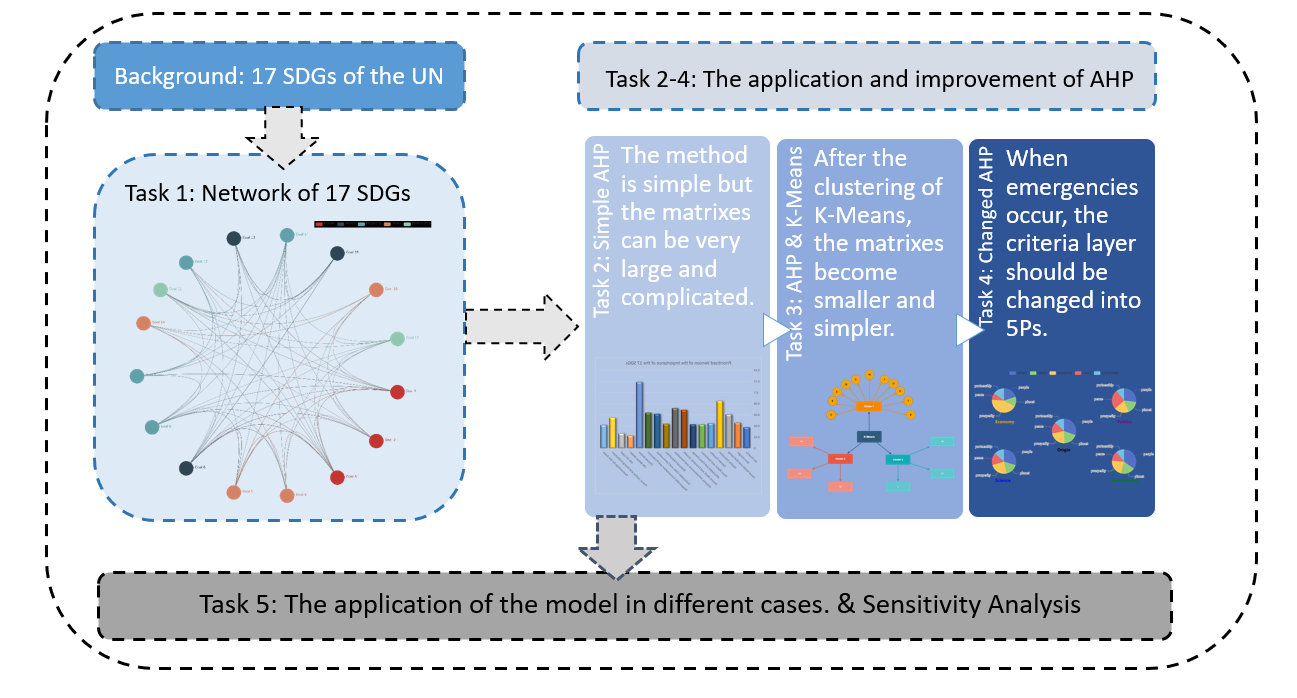
\includegraphics[scale=0.59]{{figure/LiuCheng.png}}%插入图片的指令
    \caption{Our Work Structure}%标题
    \label{Label}
\end{figure}

